\begin{figure*}[t]
  \centerline{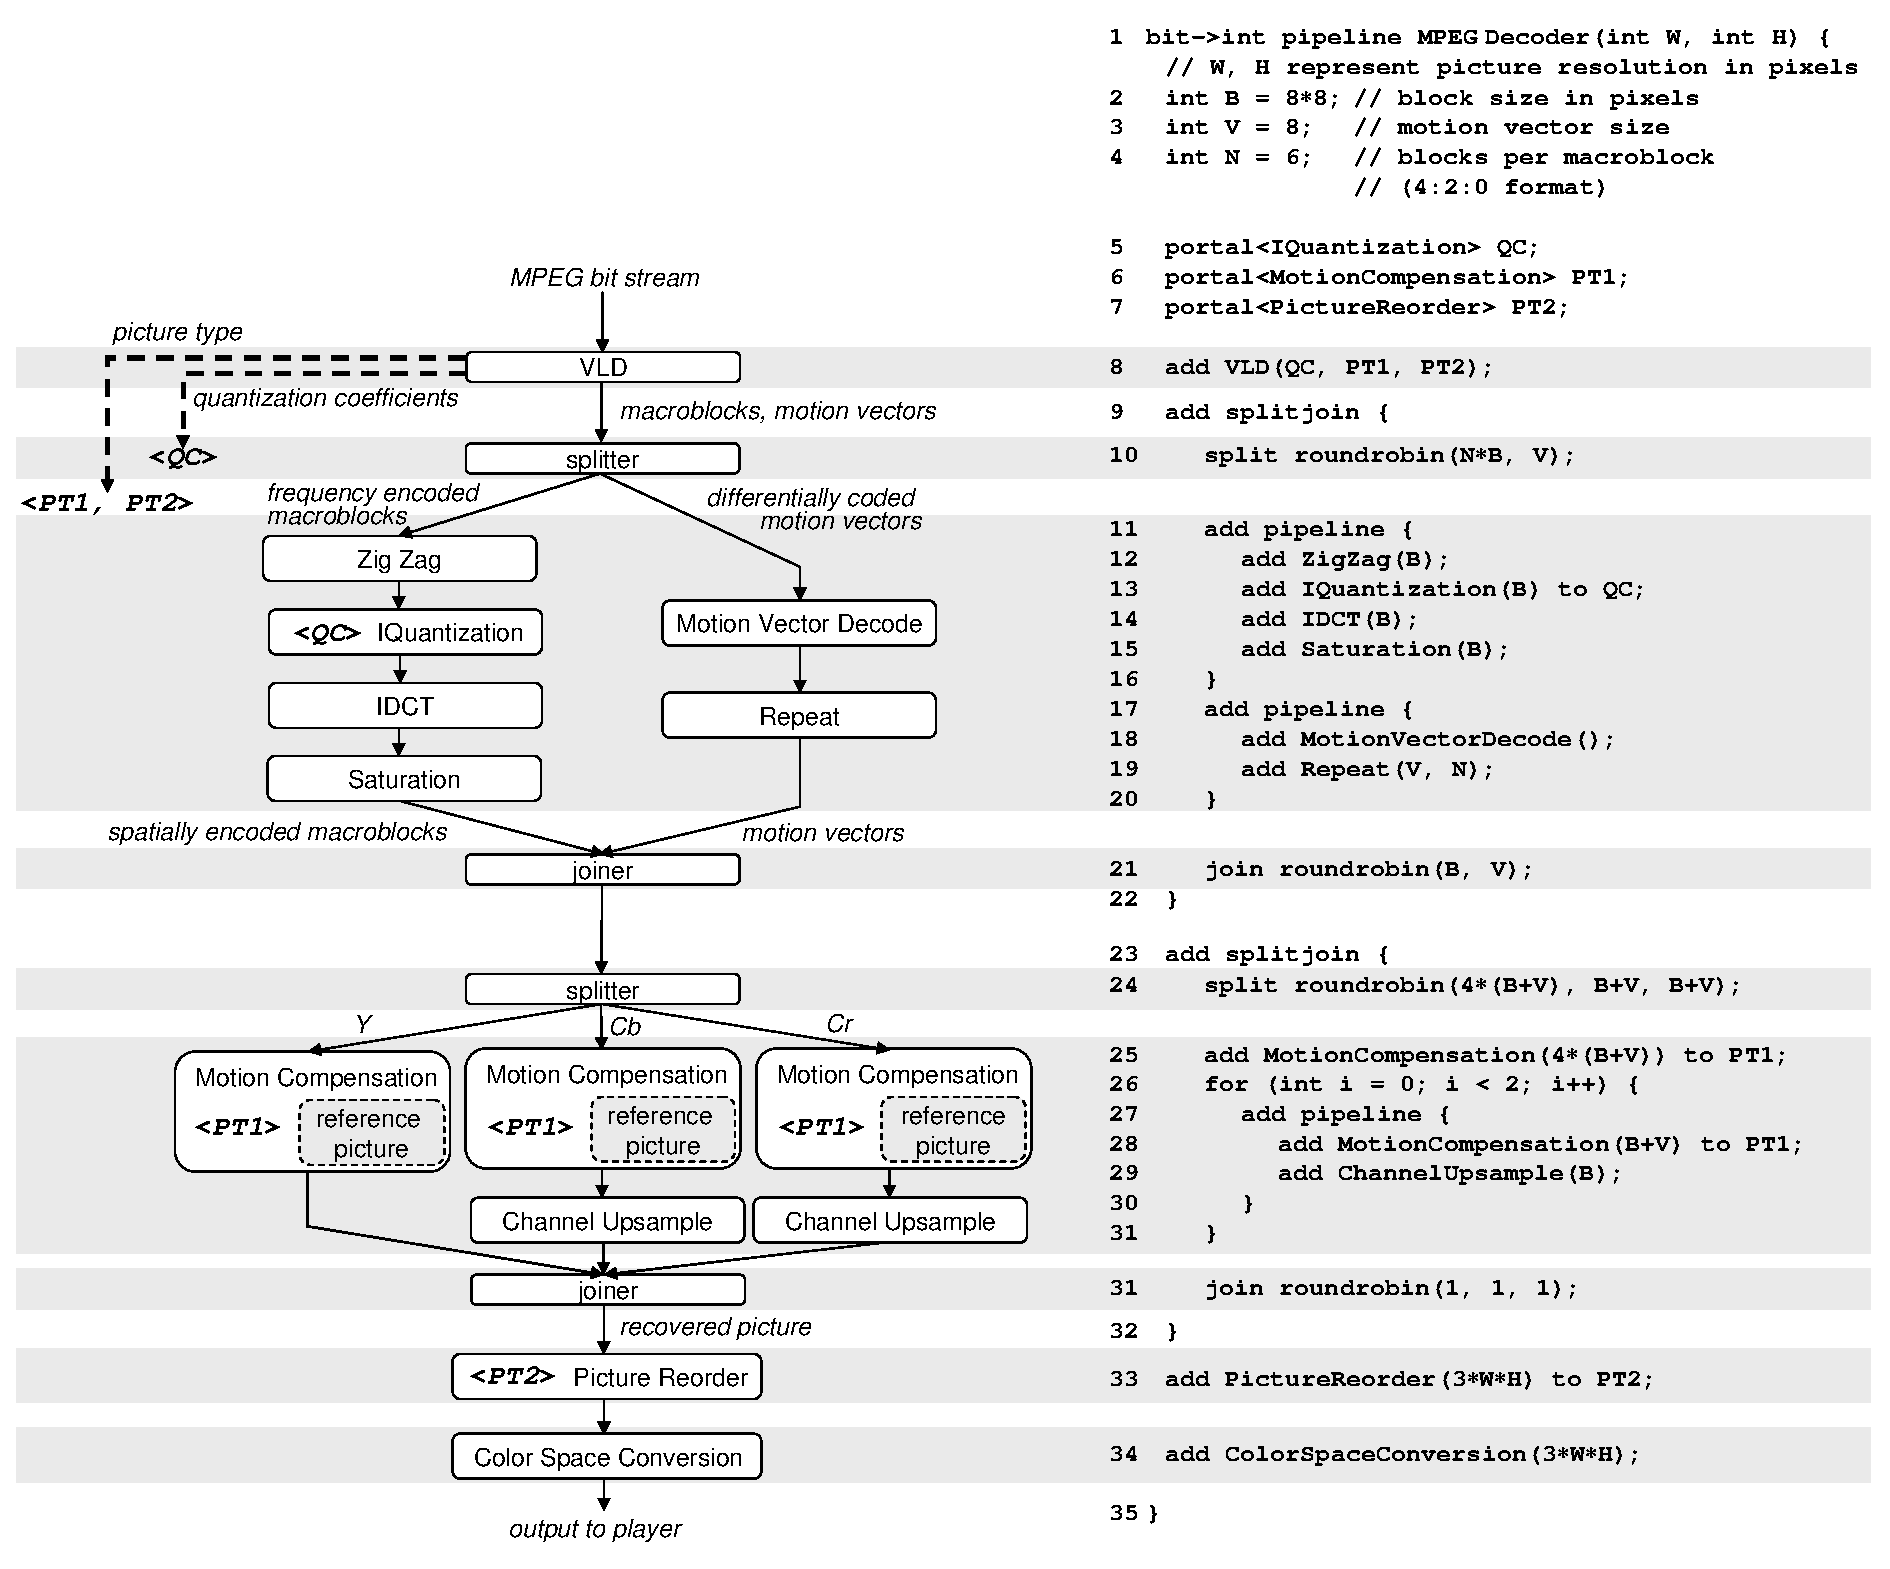
\epsfig{file=decoder_with_code.eps,width=5in}}
  \caption{MPEG-2 decoder block diagram and corresponding StreamIt code.}
  \label{fig:dec-with-code}
\end{figure*}

\Section{MPEG Decoder in StreamIt}

The MPEG decoder pipeline is shown in
Figure~\ref{fig:dec-with-code}. The stream graph is shown on the left,
alongside the StreamIt code on the right. It is worthy to note that
there is a high correlation between the stream block level diagram and
the StreamIt syntax describing the pipeline.

The decoder accepts a compressed bit stream as input, and produces the
decoded video stream as output. The computation is encapsulated in
three main components: the parser (line 5), the block and motion vector
decoder (lines 6-16), and the motion compensator (lines 17-27).

The parser is responsible for parsing the MPEG-2 bit stream and
performing Huffman and variable run-length decoding (VLD). The output
of the VLD is an interleaved stream of quantized macroblocks encoded
in the frequency-domain, and offset-encoded motion vectors. The VLD
outputs $\texttt{N}\times\texttt{B}$ data elements for each
macroblock, followed by \texttt{V} data elements that encode its
motion vector. The actual value of \texttt{N} depends on the chroma
format. In a 4:2:0 chroma format regime, $\texttt{N}=6$ since each
macroblock consists of four 8x8 subpixel blocks in the luminance channel,
and two 8x8 subpixel blocks in each of the two chrominance
channels. Therefore, the VLD outputs a total of six 8x8 blocks,
or 384 subpixels per macroblock.

The VLD output is segregated into two homogeneous streams by a
round robin splitter (line 7). The first stream undergoes inverse
transformations (lines 8-13), while the second is decoded to produce
absolute motion vectors (line 14). As is evident from the computation
graph, the two streams are decoded in parallel, and then merged (line
15) prior to the motion compensation stage of the pipeline.

The inverse transformations map each 8x8 block from the frequency
domain back to the spatially encoded domain. Each block is reordered
(line 9), and then inversely quantized (line 10). This is followed by
an inverse DCT and a bounded saturation filter (lines 11-12). The set
of transformations is grouped into an anonymous pipeline whose input
and output types are automatically inferred by the compiler. Each of
the filters in this pipeline operate on 8x8 blocks. The code that is
shown does not take advantage of data level parallelism between
blocks. It is rather straight forward however to expose this
parallelism if it is desirable. For example, in this case a splitjoin
can replicate the inverse transformation pipeline six times:
\begin{center}
\begin{verbatim}
add splitjoin {
   split roundrobin(B);
   for (int i = 0; i < 6; i++) 
      // add pipeline
   join roundrobin(B);
}
\end{verbatim}
\end{center}
A stream-aware compiler can also automatically adjust the execution
granularity as necessary~\cite{gordo-asplos}.

The third stage of the decoding pipeline performs the motion
compensation (lines 17-27) to recover predictively coded
macroblocks. The motion compensation filter uses the motion vectors to
find a corresponding macroblock in a previously decoded reference
picture. The reference macroblock is added to the current macroblock
to recover the original picture data. If the current macroblock is
part of an I or P picture, then the decoder stores it for use as a
future reference picture.

In the compensation stage, there are three parallel stream
processors. The first handles the luminance color channel (Y), and the
other two handle the chrominance channels (Cb and Cr). The round robin
splitter (line 18) distributes the macroblocks according to the chroma
format. Since the luminance channel is not down sampled during the
encoding process, the splitter dispatches four 8x8 blocks at a time to
the Y motion compensator. The chrominance channels are typically down
sampled by a factor of 4, and hence one 8x8 block is streamed to each
of the Cb and Cr pipelines, which up sample (line 23) the results of
the motion compensator to generate the full 16x16 macroblock.  The
joiner (line 26) assembles the pictures from each of the color
channels, one pixel at a time. The output is then readied for display
(lines 28 and 29) by organizing the pictures in accord with their
temporal order, and performing color space conversion to the RGB (red,
green, blue) color model. Note that these two filters each consume
$3\times\texttt{W}\times\texttt{H}$ subpixels per picture. This is three
times the pixel resolution of the decoded image since there is one
pixel generated from each of the three channel decoders. The output of
the decoder is $\texttt{W}\times\texttt{H}$ pixels in the end.

The MPEG-2 decoder in StreamIt is a fully portable implementation in
that the application is not architecture dependent. The implementation
naturally exposes the pipeline parallelism that exists throughout the
decoder, as well as the data level parallelism inherent to the inverse
transformations and motion compensation.

The implementation was carried out by one student programmer with no
prior understanding of MPEG. The development spanned eight weeks from
specification~\cite{MPEG2} to the first fully functional MPEG
decoder. The StreamIt code is nearly 3,165 lines of code with 48
static streams. The bit stream parser is the largest single filter,
consisting of 775 lines of code. The 48 static streams are compiled to
2,150 filters for a picture resolution of 352x240. By way of
comparison, the reference C implementation~\cite{reference-mpeg-c} is
6,835 lines of code. A line count comparison is not an accurate
measure of programmability, and our StreamIt decoder 
implements only a subset of several stream types supported by MPEG.
Our decoder does provide full support for the range of different 
compression techniques used within MPEG, but supports only a subset 
of the possible display modes (i.e. interlaced versus progressive output).
However, these alternate display formats represent minor conceptual
changes and should therefore affect small portions of the StreamIt code. 
This is demonstrated in Section~\ref{section:chroma} with an example of
support for multiple chrominance formats. 

The reference C implementation intermingles parsing, decoding, and
motion compensation, making it difficult to clearly follow the code,
and hinders a better comparison. The C code also relies on global
variables to communicate values, such as quantization coefficients,
from the parser to the relevant code regions. In StreamIt, such
communication is relegated to teleport messaging (lines 5, 10, 22, and
28, and illustrated with dotted lines in
Figure~\ref{fig:dec-with-code}). For instance, the parser (VLD)
generates a message whenever the picture or macroblock type
changes. The motion compensation filter receives this information via
its dedicated portal (line 22), and determines how to process the
current picture, and whether it needs to store it for future
reference. The picture reordering filters receives a similar message
(via portal on line 28), and uses the information to determine the
correct temporal order of picture. The inverse transformation pipeline
listens to its portal (line 10) to determine the algebraic
manipulation required to perform the inverse quantization of the input
macroblock. Teleport messaging proves as a natural mechanism because
the macroblock type and picture type information changes infrequently
and irregularly, compared to the regular flow of data in the
application.

In StreamIt, all of the processing is encapsulated hierarchically into
single input-single output streams with well defined modular
interfaces. This property facilitates development and boosts
programmer productivity, as components can be debugged and verified as
standalone components. The modularity also promotes reuse. For
example, the zig-zag descrambler, inverse quantizer, and inverse DCT
components may be used as is to implement a JPEG decoder.

Another noteworthy aspect of the StreamIt implementation is its
malleability. We illustrate this by outlining how the decoder
implementation, originally designed to deal with a 4:2:0 chroma
sampling rate is modified for a 4:2:2 sampling rate. MPEG-2 streams
are typically encoded using the former, which achieves a 50\%
reduction in the number of bits required to represent a
video. However, better quality is possible with higher sampling rates
since more color information is retained from the original picture. In
this sequel, we show that the migration path to support multiple
chroma formats is trivial.

\Section{Code Malleability: A Case Study}
\label{section:chroma}

To illustrate the concrete benefits of programming in a stream
language, we compare the support for varying chroma formats in the
StreamIt and C implementations.  While the conceptual difference
between chroma formats is merely a change in downsampling ratio, this
leads to a change in the data rates and the ratios of data between the
color channels. This requires that the C implementation parameterize
its buffer sizes, array lengths, array indices, and pointer offsets on
the chroma format; the reference implementation uses a ``chroma flag''
to dictate control flow to alternate index/offset calculations in 43
locations in the code. As an example, a fragment of the
``form\_prediction'' routine (in recon.c~\cite{reference-mpeg-c}) used
for motion compensation is shown in Figure~\ref{fig:chroma}. This
function calls a subroutine to perform the actual motion compensation
on each of the three color channels, passing in array offsets to a
global array holding the data. Lines 4-6 adjusts values used for
address calculations to handle the 4:2:2 and 4:2:0 chroma formats, and
lines 7-9 provide additional adjustments for the 4:2:0 format. While
these offset adjustments are necessary in C, they are difficult for
programmers and make the code hard to understand.

To add support for the 4:2:2 chroma format in our StreamIt decoder, we
modified 31 lines and added 20 new lines. Of the 31 modified lines, 23
were trivial modifications to pass a variable representing the chroma
format as a stream parameter. The greatest substantial change was to
the color channel splitter, previously illustrated on line 20 of
Figure~\ref{fig:dec0with-code}. In the case of a 4:2:2 sampling
rate, the chrominance data, as it appears on the input tape,
alternates between each of the two chrominance channels. Thus, a
nested splitjoin is used to properly recover the appropriate
chrominance channels. The new splitjoin is shown in
Figure~\ref{fig:chroma}.  Even after these modifications, the chroma
format only explicitly dictates control flow in 9 locations. Of
course, the scheduling and buffer management changes dramatically
between chroma formats, but this is automatic and hidden from the
programmer.

\begin{figure*}[t]
 \begin{minipage}[t]{4.3in}
   {
   % Matt's note - this is the C reference code I added.
   % I added the line numbers so I can reference them in the text.
    \begin{scriptsize}
    \begin{verbatim}
1    /* Y */
2    form_component_prediction(src[0]+(sfield?lx2>>1:0),dst[0]+(dfield?lx2>>1:0),
3                              lx,lx2,w,h,x,y,dx,dy,average_flag);
4    if (chroma_format!=CHROMA444)  {
5        lx>>=1; lx2>>=1; w>>=1; x>>=1; dx/=2;
6    }
7    if (chroma_format==CHROMA420)  {
8        h>>=1; y>>=1; dy/=2;
9    }
10   /* Cb */
11   form_component_prediction(src[1]+(sfield?lx2>>1:0),dst[1]+(dfield?lx2>>1:0),
12                             lx,lx2,w,h,x,y,dx,dy,average_flag);
13   /* Cr */
14   form_component_prediction(src[2]+(sfield?lx2>>1:0),dst[2]+(dfield?lx2>>1:0),
15                             lx,lx2,w,h,x,y,dx,dy,average_flag);    
    \end{verbatim}
    \end{scriptsize}
   }
   % \vspace{-3pt}
   % \caption{Decoding stream to handle 4:2:0 and 4:2:2 chroma formats.}
   % \label{fig:chroma-stream}
  \end{minipage}
    ~~\hrule~~
 \begin{minipage}[t]{4.3in}
   {
    \begin{scriptsize}
    \begin{verbatim}
    // C = blocks per chrominance channel per macroblock 
    // C = 1 for 4:2:0, C = 2 for 4:2:2
    add splitjoin {
      split roundrobin(4*(B+V), 2*C*(B+V));
      add MotionCompensation() to PT1;
      add splitjoin {
        split roundrobin(N, N);
        for (int i = 0; i < 2; i++) {
          add MotionCompensation() to PT1;
          add ChannelUpsample(C);
        }
        join roundrobin(1, 1);
      }
      join roundrobin(1, 1, 1);
    }
    \end{verbatim}
    \end{scriptsize}
   }
   % \vspace{-3pt}
   % \caption{Decoding stream to handle 4:2:0 and 4:2:2 chroma formats.}
   % \label{fig:chroma-stream}
  \end{minipage}
  ~~\vrule~~
  \begin{minipage}[t]{2.0in}
  {
   \begin{center}
    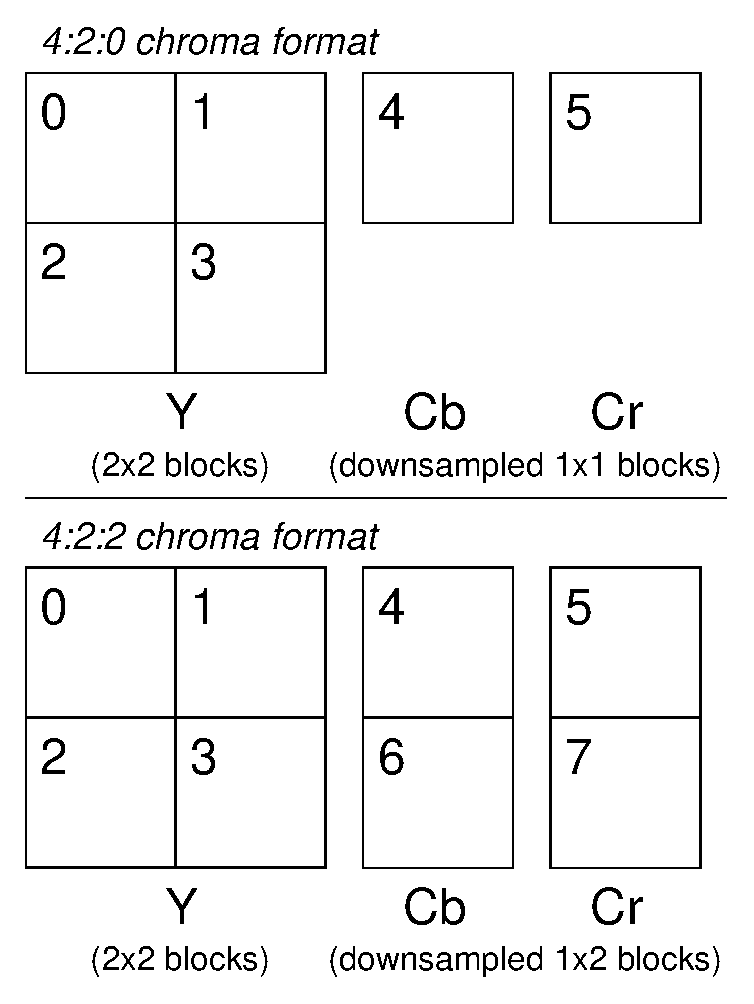
\epsfig{file=chroma_format.eps, width=2.5in}
    % \caption{4:2:0 and 4:2:2 chroma formats showing macroblock ordering}
    % \label{fig:chroma-format}
   \end{center}
  }
  \end{minipage}
  \caption{Decoding stream to handle 4:2:0 and 4:2:2 chroma
    formats. Figures on right illustrate how macroblock orderings
    differ.}
  \label{fig:chroma}
\end{figure*}

%% \SubSection{Motion Compensation}

% Commented out this section since this information is incorporated into
% the decoder implementation section. - Matt 1/25/06
% An MPEG decoder accepts a bitstream as input and performs Huffman and
% variable run-length decoding (VLD).  This process results in a set of
% quantized, frequency-domain macroblocks and corresponding motion
% vectors.  The decoder inversely quantizes (IQ) the macroblocks and then
% performs an inverse DCT (IDCT) to convert the macroblocks to the
% spatial domain.  For predictively coded macroblocks (e.g., P and B
% pictures), the decoder performs motion compensation (MC) using the
% input motion vectors to find a corresponding macroblock in a
% previously decoded, stored reference picture. This reference
% macroblock is added to the current macroblock to recover the original
% picture data. If the current macroblock is part of an I or P picture,
% then the decoder stores it for future reference.
% Figure~\ref{fig:dec_block} illustrates the decode sequence.

%\begin{figure}[htbp]
%\centerline{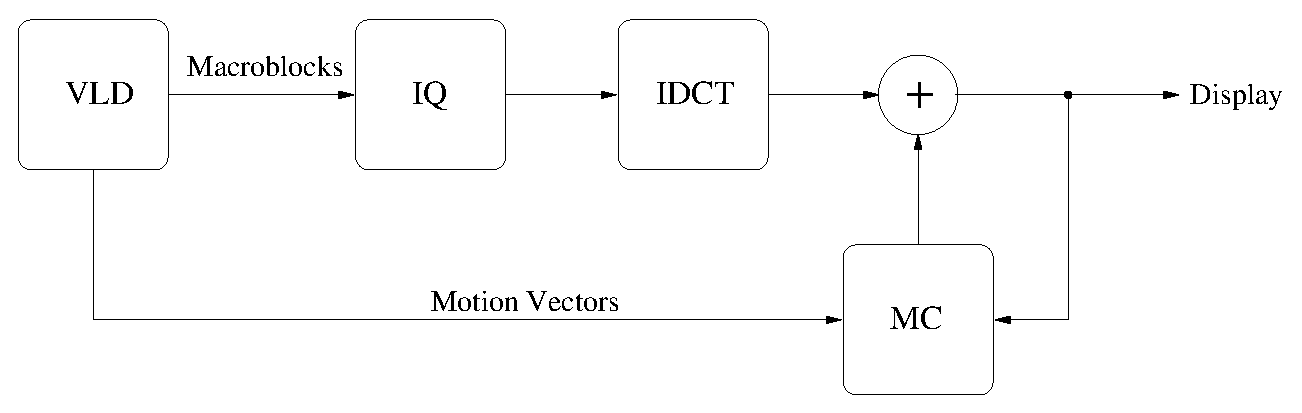
\epsfig{file=dec_block.eps,width=5in}}
%\caption{Block diagram of MPEG-2 decode.}
%\label{fig:dec_block}
%\end{figure}

%% A simple strategy for parallelizing the MPEG-2 decoding can exploit
%% the data parallelism among macroblocks. Using this scheme, the Huffman
%% and run-length decoding is inherently serial, as macroblock boundaries
%% can only be discovered by performing the decode operation.  Once this
%% decode is complete, a parallel implementation can distribute
%% macroblocks to independent streams (using a splitjoin). Each stream
%% performs the inverse quantization, inverse discrete cosine transform,
%% and motion compensation. Furthermore, each stream locally stores
%% reference macroblocks for future motion compensation. Using this
%% strategy, the streams can execute independently with one exception.

%% % TODO: This is the figure showing the macroblock parallelism
%% % I'm not sure where it goes. - Matt
%% \begin{figure*}[t]
%% \vspace{-12pt}
%% %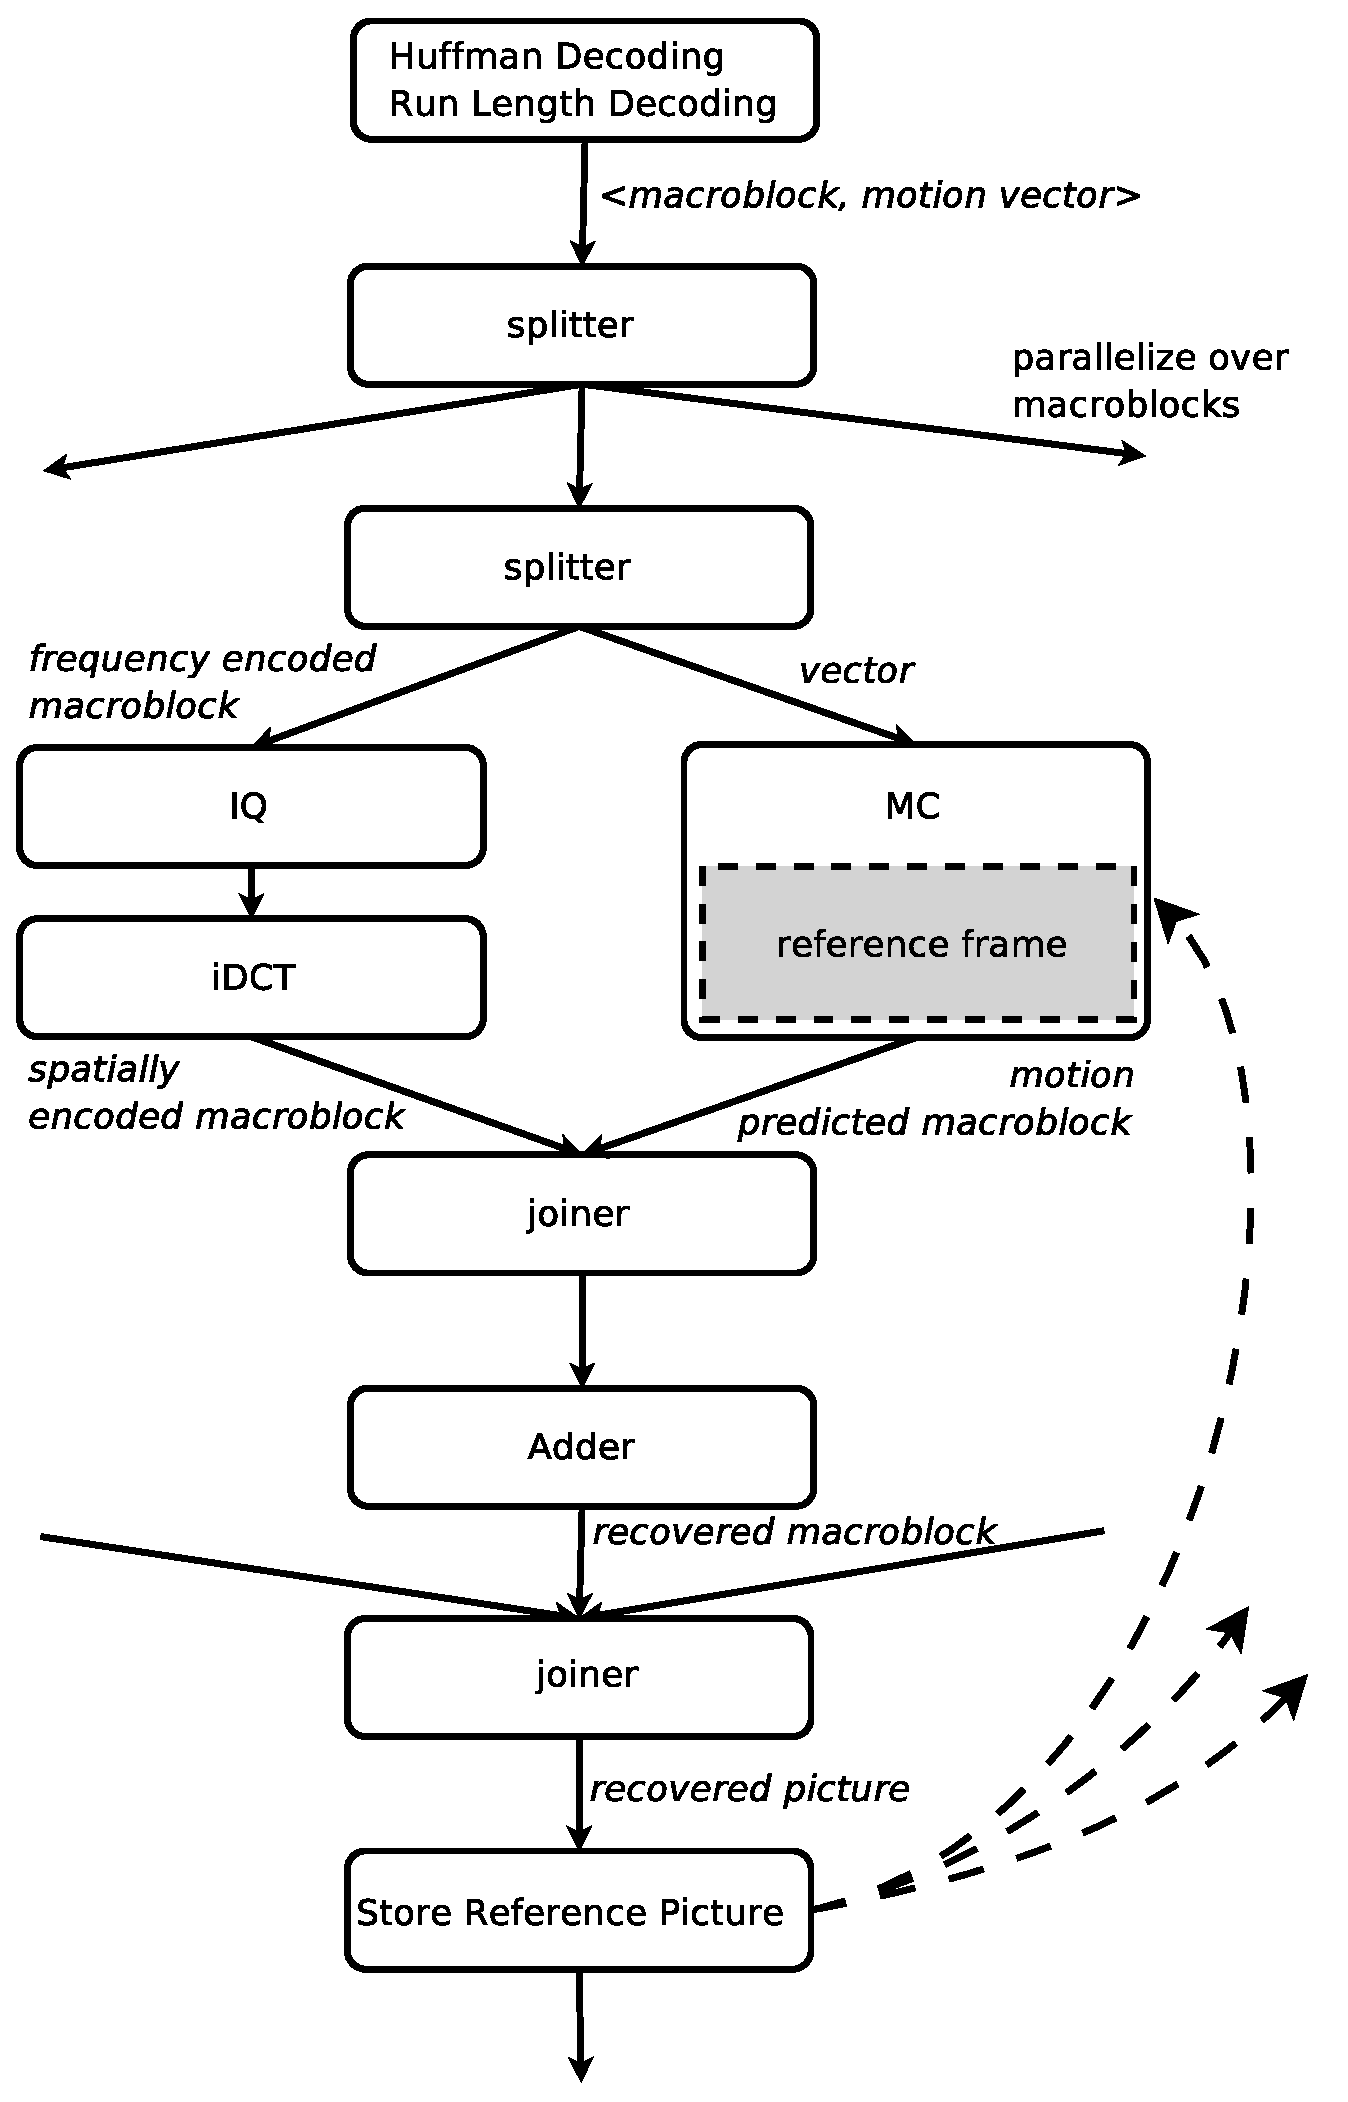
\epsfig{file=decoder_macroblock_parallelism.eps, width=3in}
%% %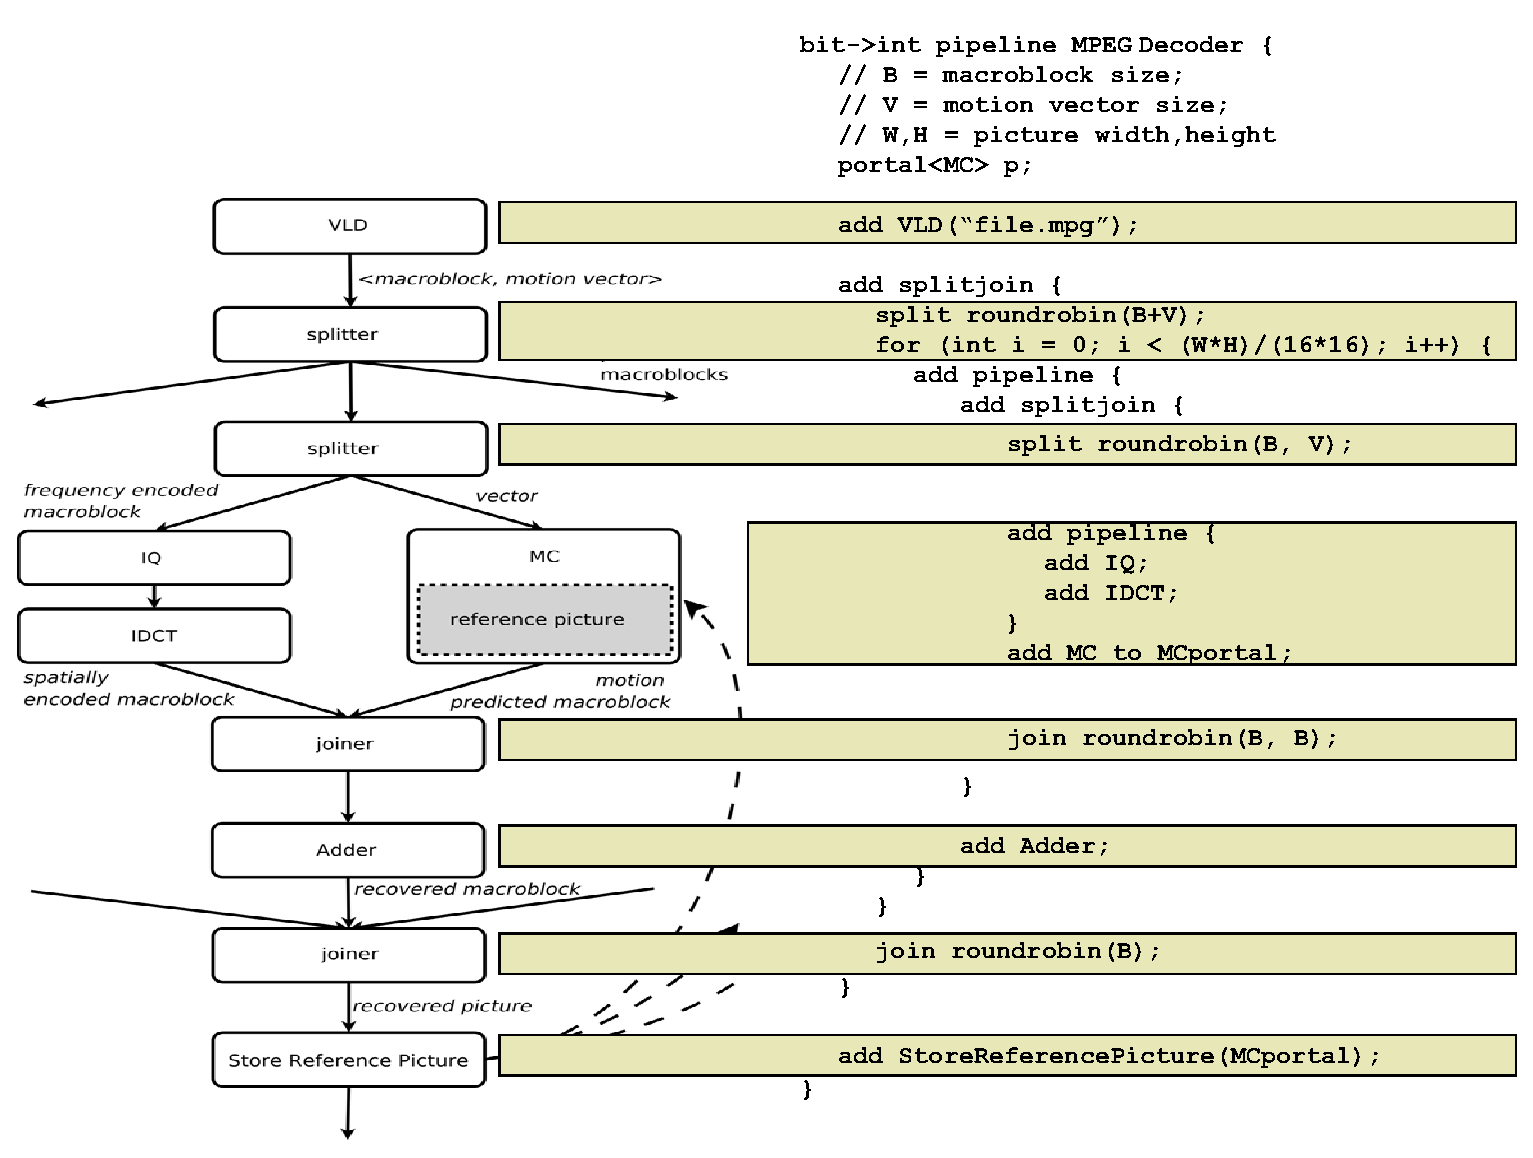
\epsfig{file=decoder-parallel.eps, width=\textwidth}
%% 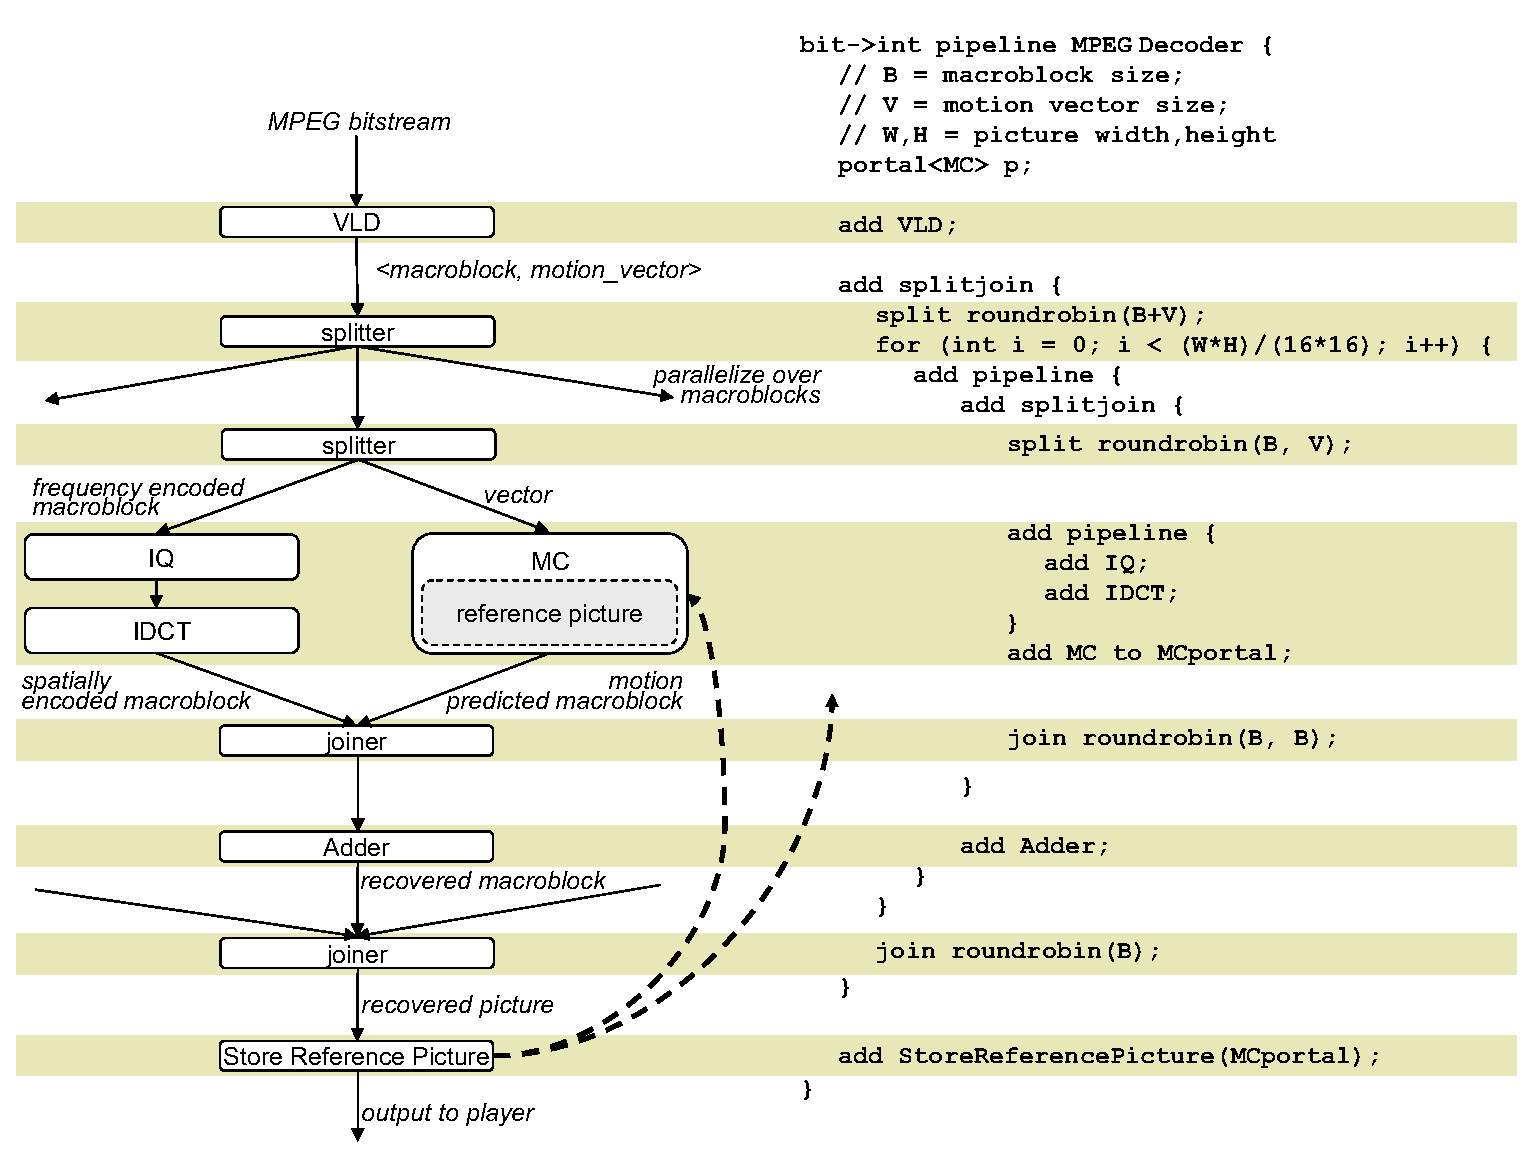
\epsfig{file=decoderpipeline.eps, width=\textwidth}
%% % TODO: Change Matt's 2 am caption.
%% \caption{MPEG-2 decoder exploiting macroblock-level parallelism.}
%% \label{decoder_macroblock_parallelism}
%% \vspace{-6pt}
%% \end{figure*}

%% This exception occurs when a stream is performing motion compensation
%% and the corresponding motion vector indicates a reference macroblock
%% stored in some other stream. In this case, inter-stream communication
%% is required to send the reference data to the requesting stream. This
%% situation is not uncommon, and is more prevalent for higher resolution
%% pictures. A simple scheme for handling this situation is for every
%% stream to broadcast its decoded macroblocks to all other streams. This
%% solution has the benefit of being conceptually easy to understand and
%% implement. StreamIt allows programmers to naturally expose such
%% parallelism.
%% A StreamIt pipeline that operates at macroblock
%% granularity is shown in Figure~\ref{decoder_macroblock_parallelism}. It is
%% worthy to note that there is a high correlation between the stream
%% graph, and the StreamIt syntax describing the pipeline.

%% The implementation can be made more fine grained by exposing the
%% intra-macroblock parallelism. For example, the IQuantization-IDCT
%% pipeline can operate at a block level, rather than at a macroblock
%% granularity. This is easily achieved by encapsulating the  pipeline
%% within a splitjoin to scatter the blocks, operate, and gather the
%% results to recover the parent macroblock.

%% There are many implementation strategies for the decoder, each with
%% varying degrees of exposed parallelism. Of the greatest advantage of
%% the StreamIt implementation is its malleability. The stream graph is
%% easily reconfigured to operate at picture-level granularity (exposing
%% parallelism between chroma channels), macroblock level (exposing even
%% more data-level parallelism), or even at block level (exposing the
%% greatest amount of data-level parallelism).